%Dokumentklasse
\documentclass[a4paper,12pt]{scrreprt}
\usepackage[left = 2.5cm, right = 2cm, bottom = 4 cm]{geometry}
%\usepackage[onehalfspacing]{setspace}
% ============= Packages =============

% Dokumentinformationen
\usepackage[
	pdftitle={Seminararbeit_1126113},
	pdfsubject={},
	pdfauthor={Christoph Weichselbaum, Christof Kocer},
	pdfkeywords={}
	pdftex=true, 
	colorlinks=true,
 	breaklinks=true,
	citecolor=black,
	linkcolor=black,	
	menucolor=black,	
	urlcolor=black
]{hyperref}

% Standard Packages
\usepackage[utf8]{inputenc}
\usepackage[ngerman]{babel}
\usepackage[T1]{fontenc}
\usepackage{graphicx}
\usepackage{graphicx, subfigure}
\graphicspath{{img/}}
\usepackage{fancyhdr}
\usepackage{lmodern}
\usepackage{color}
\usepackage{transparent}
\usepackage{float}
\usepackage{verbatim}
\usepackage{titlesec}
\usepackage{changepage}
\usepackage{listings}
\usepackage{color}
\usepackage{setspace}
\usepackage[authoryear]{natbib}


% ============= Nummerierung der Subsubsections ============= 
\setcounter{secnumdepth}{3}
\setcounter{tocdepth}{3}

% ============= Überschriftenformatierung ============= 
\titleformat*{\section}{\LARGE\bfseries}
\titleformat*{\subsection}{\Large\bfseries}
\titleformat*{\subsubsection}{\large\bfseries}
\titleformat*{\paragraph}{\large\bfseries}
\titleformat*{\subparagraph}{\large\bfseries}

% ============= Diagrammoptionen ============= 
\usepackage{tikz}
\usetikzlibrary{arrows,shapes,positioning,shadows,trees,decorations.markings}

% zusätzliche Schriftzeichen der American Mathematical Society
\usepackage{amsfonts}
\usepackage{amsmath}

% nicht einrücken nach Absatz
\setlength{\parindent}{0pt}

% ============= Redefinition von fancy ============= 
\fancypagestyle{plain}{
  \fancyhf{}
  \fancyfoot[R]{\thepage}
  \renewcommand{\headrulewidth}{0pt}
}
\fancyhf{}
\fancyhead[R]{\slshape \leftmark}
\fancyfoot[R]{\thepage}
\renewcommand{\headrulewidth}{0.4pt}
\renewcommand{\footrulewidth}{0pt}

% ============= Package Einstellungen & Sonstiges ============= 

%Besondere Trennungen
%\hyphenpenalty=10000
\hyphenation{De-zi-mal-tren-nung St-rei-fen-licht-scan-nern}

%römische Aufzählungen mit \RM{Zahl}
\newcommand{\RM}[1]{\MakeUppercase{\romannumeral #1}}

% ============= Code Style ============= 
\definecolor{mygreen}{rgb}{0,0.6,0}
\definecolor{mygray}{rgb}{0.5,0.5,0.5}
\definecolor{mymauve}{rgb}{0.58,0,0.82}

\lstset{literate=%
  {Ö}{{\"O}}1
  {Ä}{{\"A}}1
  {Ü}{{\"U}}1
  {ß}{{\ss}}2
  {ü}{{\"u}}1
  {ä}{{\"a}}1
  {ö}{{\"o}}1
}

\lstset{ %
  backgroundcolor=\color{white},   % choose the background color; you must add \usepackage{color} or \usepackage{xcolor}
  basicstyle=\footnotesize,        % the size of the fonts that are used for the code
  breakatwhitespace=false,         % sets if automatic breaks should only happen at whitespace
  breaklines=true,                 % sets automatic line breaking
  captionpos=b,                    % sets the caption-position to bottom
  commentstyle=\color{mygreen},    % comment style
  deletekeywords={...},            % if you want to delete keywords from the given language
  escapeinside={\%*}{*)},          % if you want to add LaTeX within your code
  extendedchars=true,              % lets you use non-ASCII characters; for 8-bits encodings only, does not work with UTF-8
  frame=single,                    % adds a frame around the code
  keepspaces=true,                 % keeps spaces in text, useful for keeping indentation of code (possibly needs columns=flexible)
  keywordstyle=\color{blue},       % keyword style
  language=Octave,                 % the language of the code
  morekeywords={*,...},            % if you want to add more keywords to the set
  numbers=left,                    % where to put the line-numbers; possible values are (none, left, right)
  numbers=none,
%  numbersep=5pt,                   % how far the line-numbers are from the code
%  numberstyle=\tiny\color{mygray}, % the style that is used for the line-numbers
%  rulecolor=\color{black},         % if not set, the frame-color may be changed on line-breaks within not-black text (e.g. comments (green here))
  showspaces=false,                % show spaces everywhere adding particular underscores; it overrides 'showstringspaces'
  showstringspaces=false,          % underline spaces within strings only
  showtabs=false,                  % show tabs within strings adding particular underscores
  stepnumber=2,                    % the step between two line-numbers. If it's 1, each line will be numbered
  stringstyle=\color{mymauve},     % string literal style
  tabsize=2,                       % sets default tabsize to 2 spaces
  title=\lstname,                   % show the filename of files included with \lstinputlisting; also try caption instead of title
  mathescape=true
}



% ============= Dokumentbeginn =============

\begin{document}

\pagestyle{empty}
\begin{center}
\begin{tabular}{p{\textwidth}}


\begin{center}

\includegraphics[scale=0.9]{img/TU_Vienna.jpg}
\end{center}


\\

\begin{center}
\large{\textsc{
Sighted! - die mobile Lösung für das interaktive Mapping von Gebäuden
}}
\end{center}

\\


\begin{center}
\normalsize{Fakultät für Mathematik und Geoinformation \\
am \\
Department für Geodäsie und Geoinformation \\
der Technischen Universität Wien \\}
\end{center}

\\

\begin{center}
\textbf{\Large{Technischer Bericht}}
\end{center}

\begin{center}
vorgelegt von
\end{center}

\begin{center}
\large{\textbf{Christoph Weichselbaum, 1126113}} \\
\large{\textbf{Christof Kocer, 1026228}} \\
\end{center}

\begin{center}
\large{am 29. Februar 2016}
\end{center}

\end{tabular}
\end{center}

% \part im Inhaltsverzeichnis nicht nummerieren
\makeatletter
\let\partbackup\l@part
\renewcommand*\l@part[2]{\partbackup{#1}{}}

%Seitennummerierung neu beginnen, Zahlen [arabic], röm.Zahlen [roman,Roman], Buchstaben [alph,Alph]
\pagenumbering{Roman}
\pagestyle{fancy}% Fancy page style

\newpage
%Inhaltsverzeichnis
\tableofcontents

\newpage
%Seitennummerierung neu beginnen, Zahlen [arabic], röm.Zahlen [roman,Roman], Buchstaben [alph,Alph]
\pagenumbering{arabic}

\newpage
%\begingroup
%\let\clearpage\relax
\chapter{Einleitung}
\label{chp:einleitung}

Im Rahmen der LVA Mobile GIS Anwendung wird eine Applikation entwickelt. Dabei sollen alle während des Semesters gelernten elementaren Bestandteile einer mobilen Anwendung in Betracht gezogen werden. Es soll, unter Verwendung von gängigen Web-Technologien, speziell auf die Bedürfnisse von mobilen Anwendungen eingegangen werden.

\section{Entwicklungsziele}
\label{sec:ziele}

Auf Basis der im Semesterstoff erarbeiteten Lehrziele, soll die fertige Lösung folgende elementare Komponenten implementieren.

\begin{itemize}
  \setlength{\itemsep}{1pt}
  \setlength{\parskip}{0pt}
  \setlength{\parsep}{0pt}
  
  \item Verwendung einer gängigen Javascript-API für responsive mobile Design
  \item Verwendung der Overpass-API für die Abfrage von OSM-Daten
  \item Feature-Implementierung unter der Verwendung der Smartphone-Sensorik
  \item Datenbankanbindung an CouchDB
  \item Offline-Synchronisation der gespeicherten Daten
  
\end{itemize}

Des weiteren wurde bei der Implementierung stets auf folgende Unterpunkte geachtet.

\begin{itemize}
  \setlength{\itemsep}{1pt}
  \setlength{\parskip}{0pt}
  \setlength{\parsep}{0pt}
   
  \item Implementierung des MVC-Pattern
  \item Modularisierte Architektur
  \item Skallier- und Erweiterbarkeit
  \item Konfigurierbarkeit
  \item Automatisiertes Assembling der Android-APK Datei
  
\end{itemize}

\section{Methodik}
\label{sec:methodik}



Die Entwicklungsziele bilden die Grundlage und Rahmenbedingungen zur Implementierung für den Entwurf einer Android-Applikation namens 'Sighted!'. Die Methodik zur Entwicklung der vorgestellten Problemstellung umfasst folgende Punkte:

\begin{itemize}
  \setlength{\itemsep}{1pt}
  \setlength{\parskip}{0pt}
  \setlength{\parsep}{0pt}
  
  \item Aufsetzen einer Hybriden-Android Applikation, die den Zugriff auf hardwarenahe Sensorikfunktionen mittels Javascript ermöglicht.
  \item Konfiguration des Assembling-Prozesses der Applikation mittels Gradle
  \item Aufsetzen der grundlegenden Projektstruktur der Web-Applikation
  \item Konfiguration der Web-Applikation mittels Grunt
  \item Einbindung von gängigen Web-Frameworks: jquery (mobile), bootstrap, requireJS, ol3, pouchdb
  \item Implementierung des Grundgerüsts der Web-Applikation
  \item Implementierung eines Wrappers für die Verwendung der Overpass-API
  \item Implementierung eines Wrappers für die Verwendung der pouchDB-API
  \item Implementierung der Anwendungslogik und Design der Anwendung 

\end{itemize}

\chapter{Technolien}
\label{chap:technologien}

Im Rahmen der Implementierung der Anwendung werden eine Reihe von Frameworks und APIs verwendet um die Anwendungslogik effizient nach gängigen Patterns zu strukturieren. Dies ist besonders hilfreich, wenn man - wie auch im Enterpris-Umfeld - im Team an Projekten arbeitet. Die Teammitglieder können sich auf die Feature-Entwicklung konzentrieren und müssen sich nicht mit komplexen internen Anwendungsprozessen beschäftigen (e.g Templating-Engine), die bestimmte Frameworks out-of-the-box unterstützen.


\section{Back-End}
\label{sec:backend}
Das Endprodukt soll eine hybride Android-Applikation sein. Da diese Applikation lediglich auf den GPS-Sensor des Smartphones zugreift und keine komplexen hardwarenahen Operationen ausführt, wird die WebView-API von Android verwendet. Aus diesem Grund müssen die Webinhalte von einem internen Assets-Ordner aus geladen werden. Dieser Prozess wird mittels des Build-Management-Tools Gradle automatisiert. 

\subsection{Gradle}
\label{subsec:gradle}
Gradle ist ein auf Java basierendes Build-Management-Tool und wurde für Builds von Softwaresystemen entworfen. Besonders während der Entwicklungszeit werden sehr viele Änderungen am Quellcode vorgenommen, was eine ständiges Kopieren von neu erstellten Dateien in den Assets-Ordner bedeuten würde. Gradle ermöglicht es nur die Teile einer Software zu bauen, welche verändert wurden oder auf veränderten Teilen beruhen. Des weiteren können bestimmte Tasks angelegt werden, die beim Build parallel laufen (e.g. Tests). Resultat ist eine wesentlich höhere Geschwindigkeit beim Entwicklungsprozess.

\subsection{WebView}
\label{subsec:webview}
Bei WebView handelt es sich um eine Java-Klasse, die das Rendering von Webinhalten ermöglicht. Es verwendet die WebKit rendering engine für die Darstellung und implementiert Basisfunktionen eines Webbrowsers.


\section{Front-End}
\label{sec:frontend}
Während der Entwicklung werden die Vorteile von Web-Technologien ausgenützt. Anstatt jedes mal die Inhalte in die Android-Applikation zu laden und die Software dort zu testen, wird ein eigenes Submodul angelegt und das Front-End-Build-Management-Tool Grunt integriert. Des weiteren werden gängige APIs wie requireJS, jquery-mobile, bootstrap für die Anwendungslogig und Responsive-Design integriert. Für die Datenbankanbindung wird pouchDB und für die Abfrage von Geodaten wird ol3 integriert.

\subsection{Grunt}
\label{subsec:grunt}
Grunt ist ein auf node.js basierender Taskrunner und ermöglicht es eine Vielzahl an Plugins zu Nutzen, die die Entwicklung vereinfachen und beschleunigen. Im Rahmen dieser Applikation wird speziellen von der Browser-Synchronisation Gebrauch gemacht. Dabei werden Änderungen im Quellcode sofort im Browser reflektiert. Die auszuführenden Tasks werden mittels einer zentralen Konfigurationsdatei (gruntfile.js) initialisiert. 

\subsection{requireJS}
\label{subsec:requirejs}
Eine freie Javascript API für die Implementierung von asynchroner Moduldefinition (AMD). Dies ermöglicht die objektorientierte Codestrukturierung und das Laden der Dateien, wenn sie wirklich im Browser benötigt werden.

\subsection{jQuery Mobile}
\label{subsec:jquery}
Eine freie Javascript API, die DOM-Navigation und - Manipulation speziell für mobile Anwendungen optimiert. Diese API wird im Rahmen der Applikation speziell für die Navigation und bestimmte Design-Elemente verwendet.

\subsection{Bootstrap}
\label{subsec:jquery}
Eine freie Javascript API für die gezielte Manipulation von CSS-Elementen. Diese API wird im Rahmen der Applikation speziell für bestimmte Design-Elemente verwendet.

\subsection{PouchDB}
\label{subsec:pouchdb}
Eine freie Javascript API die für die Ergänzung der CouchDB API zur Unterstützung von Offline-Funktionalitäten verwendet wird. Die API läuft im Browser und speichert die Dokumente im Web Storage des Browsers.

\subsection{Overpass}
\label{subsec:overpass}
Eine freie Javascript API für die gezielte Abfrage von OpenStreetMap-Daten. Diese API wird im Rahmen der Applikation speziell für die Abfrage von Gebäudeattributen verwendet.



\chapter{Datemanagement}
\label{chap:datenmanagement}

INTRO

\section{Datenmodel}
\label{sec:datenmodel}

Wie schaut unser Datenmodell am client aus.
Wie schaut unser Datenmodell in coouchdb aus

Wie schaut das Mapping aus?

\section{Prozess der Abfrage}
\label{sec:abfrage}
welche prozesse werden durchlaufen

\section{Prozess der Speicherung}
\label{sec:speicherung}
welche prozesse werden durchlaufen


% BSP FÜR LADEN EINES BILDES
%\begin{figure}[H]
%  \centering  
%  \includegraphics[scale=0.5]{img/mapping.png}
%  \caption{Mapping CSV- zu Tabellen-Schemata}
%  \label{fig:mapping}
%\end{figure}


\chapter{Implementierung}
\label{chap:implementierung}

Die Implementierung stützt sich auf die in \ref{sec:ziele} definierten Entwicklungsziele. Zuerst soll auf die Projektstruktur und das Assembling eingegangen werden. Danach wird die Integration verschiedener APIs und die eigentliche Anwendungs-Architektur besprochen. 


\section{Projektstruktur und Assembling}
\label{sec:struktur}

Die Anwendung wird in zwei grundlegende Module gegliedert. Diese bilden das Back-End und Front-End und sind anhand Graphik  \\

\begin{figure}[H]
  \centering  
  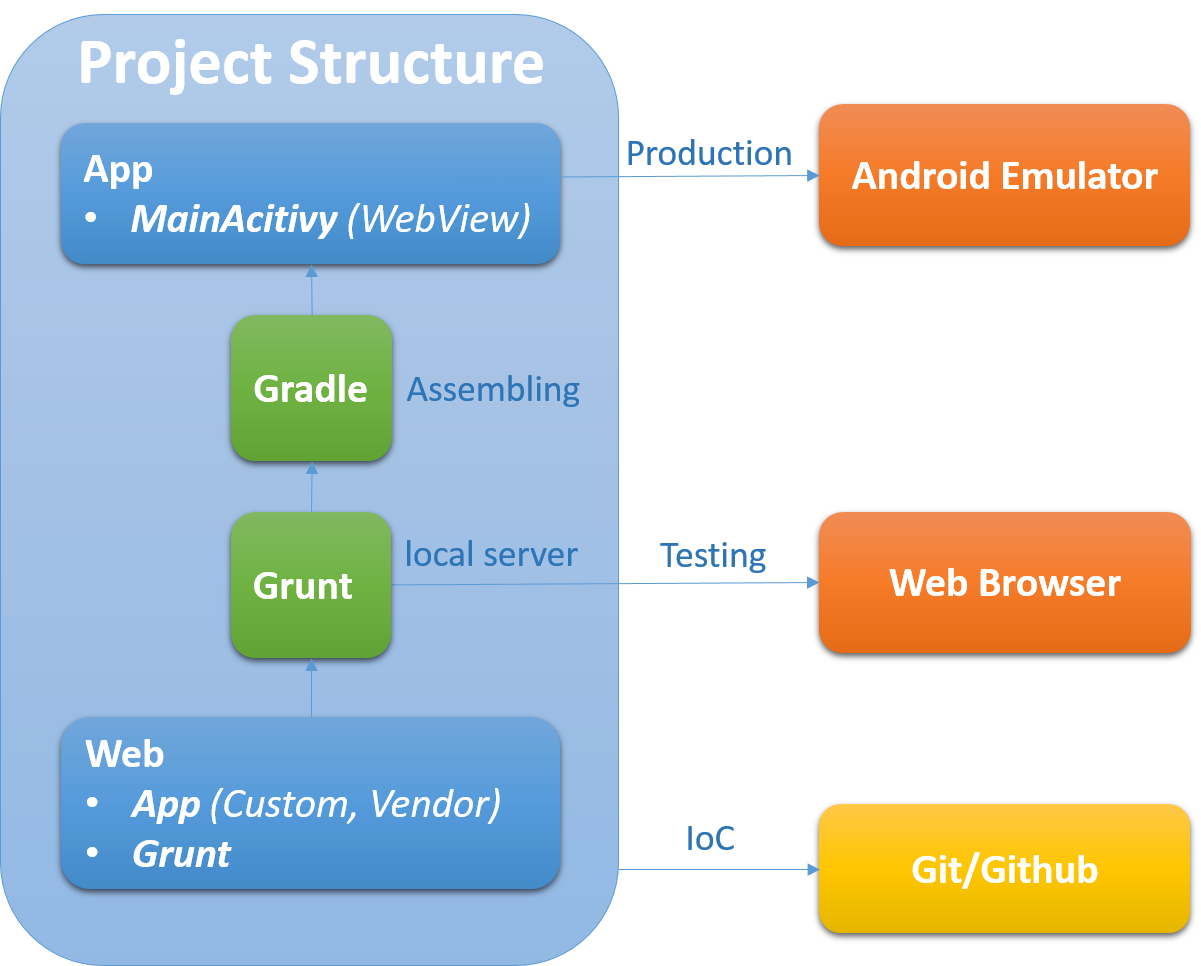
\includegraphics[scale=0.5]{img/project.png}
  \caption{Sighted! - Projektstruktur}
  \label{fig:mapping}
\end{figure}

Das erste Modul 'App' bildet das Back-End. Dieses startet das Hauptprogramm mittels der Java-Klasse MainActitivy. Dort wird der Webview initialisiert und verschiedene hardwarenahe Konfigurationen getroffen. Zu diesen Konfigurationen zählen beispielsweise bereitgestellt Rechte, die die Steuerung der Anwendung durch Javascript betreffen. \\
Das zweite Modul 'Web' bildet das Front-End. Dort werden alle Inhalte des Web-Projekts gespeichert, wie Anwendungslogik und verschiedene Javascript-APIs. Dieses Modul kann direkt mittels eines bereitgestellten HTTP-Servers in den Browser geladen werden. Speziell für Entwicklungszwecke wurde der vom Build-Management-Tool Grunt zur Verfügung gestellte HTTP-Server verwendet. Dieser erlaubt durch Browser-Synchronisation eine direkte Reflektion von geändertem Quellcode im Browser. Die hauptsächliche Entwicklung der Anwendungslogik findet auf diese Weise statt. \\
Für das Laden des Webinhalts des Front-End-Moduls in das Back-End-Modul wird das Build-Management-Tool Gradle verwendet. Es wurde ein Task definiert, der die Webinhalte automatisiert in den Assets-Ordner der Android-Applikation lädt und eine ausführbare Android-APK Datei liefert. \\
Da die Entwicklung hauptsächlich im Team stattfindet, wird das Versionsverwaltungssystem Git in Kombination mit Github verwendet. Dort sind alle Beiträge zum Projekt dokumentiert. \\

\textit{GitHub-Link}: \\
\href{https://github.com/ChriWe/MobileGIS}{https://github.com/ChriWe/MobileGIS}


\section{Architektur}
\label{sec:architektur}

Die Architektur der Anwendung folgt dem Model-View-Controller Pattern. Dabei wurden logisch unabhängige Teile des Quellcodes physisch getrennt um die Anwendung zu modularisieren. Dies soll in weiterer Folge die Skallier- und Erweiterbarkeit gewährleisten. 

\subsection{MVC-Pattern}
\label{subsec:mvc}

Das MVC-Pattern wird als Strukturierungsmodell verwendet um die Einheiten des Datenmodells, der Programmsteuerung und der Präsentation voneinander zu trennen. Ziel ist ein flexibler Programmentwurf, der spätere Änderungen oder Erweiterungen erleichtert und die Wiederverwendbarkeit von Einzelkomponenten gewährleistet. Die Geschäftslogik wird in dieser Applikation weitestgehend im Controller implementiert. \\
Die grundlegende Vorgehensweise des Musters wird anhand folgender Graphik verdeutlicht:

\begin{figure}[H]
  \centering  
  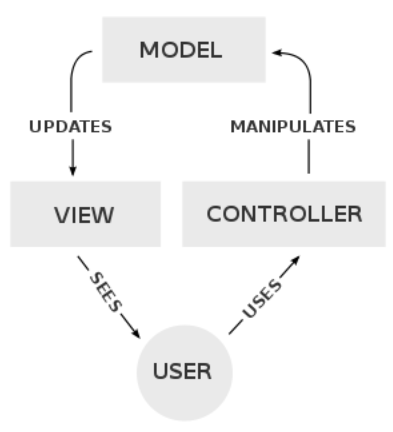
\includegraphics[scale=0.5]{img/mvc.png}
  \caption{MVC - Pattern}
  \label{fig:mapping}
\end{figure}

\begin{itemize}
  \setlength{\itemsep}{1pt}
  \setlength{\parskip}{0pt}
  \setlength{\parsep}{0pt}
  
  \item Model: enthält die zur Verfügung gestellten Daten
  \item View: ändert die Präsentation anhand von Änderungen im Model
  \item Controller: Manipuliert das Model und die View 
\end{itemize}


\subsection{Eintrittspunkt}
\label{subsec:eintrittspunkt}

Als Eintrittspunkt zur Anwendung wird eine Datei index.html definiert. Diese implementiert require.js zur Einbindung aller Javascript-Dateien und index.css zur Einbindung aller Stylesheets. \\
Für die Konfiguration von require.js wird die Datei main.js definiert, welche für das Mapping von Dateipfaden zu Namespaces zuständig ist. Die Namespaces können dann mittels asynchroner Moduldefinition dort initialisiert werden wo sie gerade gebraucht werden. Mittels requireJS werden sämtliche APIs und auch die spezifischen Anwendungsdateien initialisiert.

\subsection{Model}
\label{subsec:model}



\subsection{View}
\label{subsec:view}



\subsection{Controller}
\label{subsec:controller}











\chapter{Diskussion}
\label{sec:diskussion}

 

%\endgroup

%Verzeichnis aller Bilder
\newpage
\listoffigures

\end{document}
